% Editable native annotations around unchanged verified IDE photographs.
\par
\begin{figure}[htbp]
  \centering
  \newsavebox{\MARScrcstreamingregistersBox}
  \sbox{\MARScrcstreamingregistersBox}{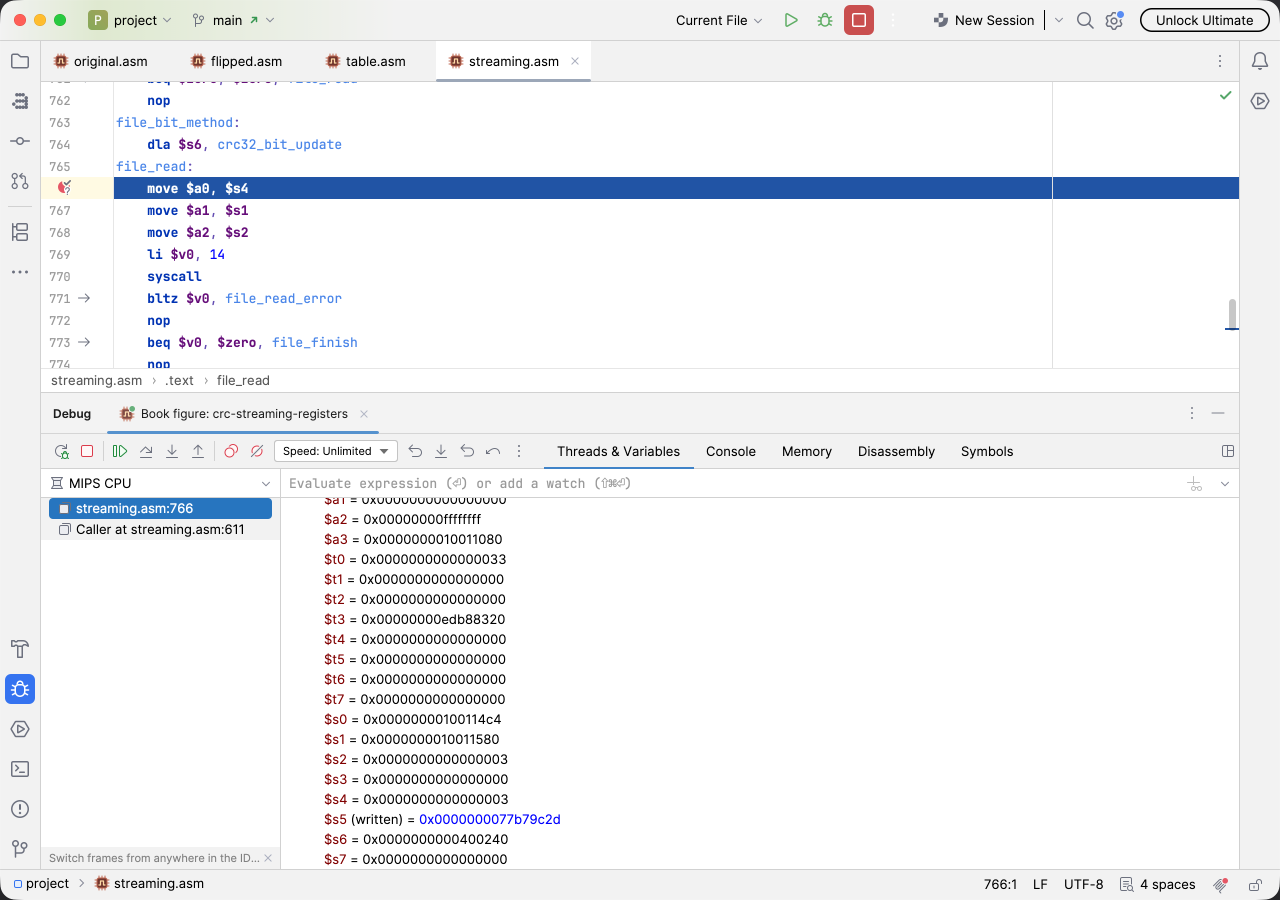
\includegraphics[artifact]{book/captures/024-crc32/f03/registers.png}}
  \newsavebox{\MARScrcstreamingscratchBox}
  \sbox{\MARScrcstreamingscratchBox}{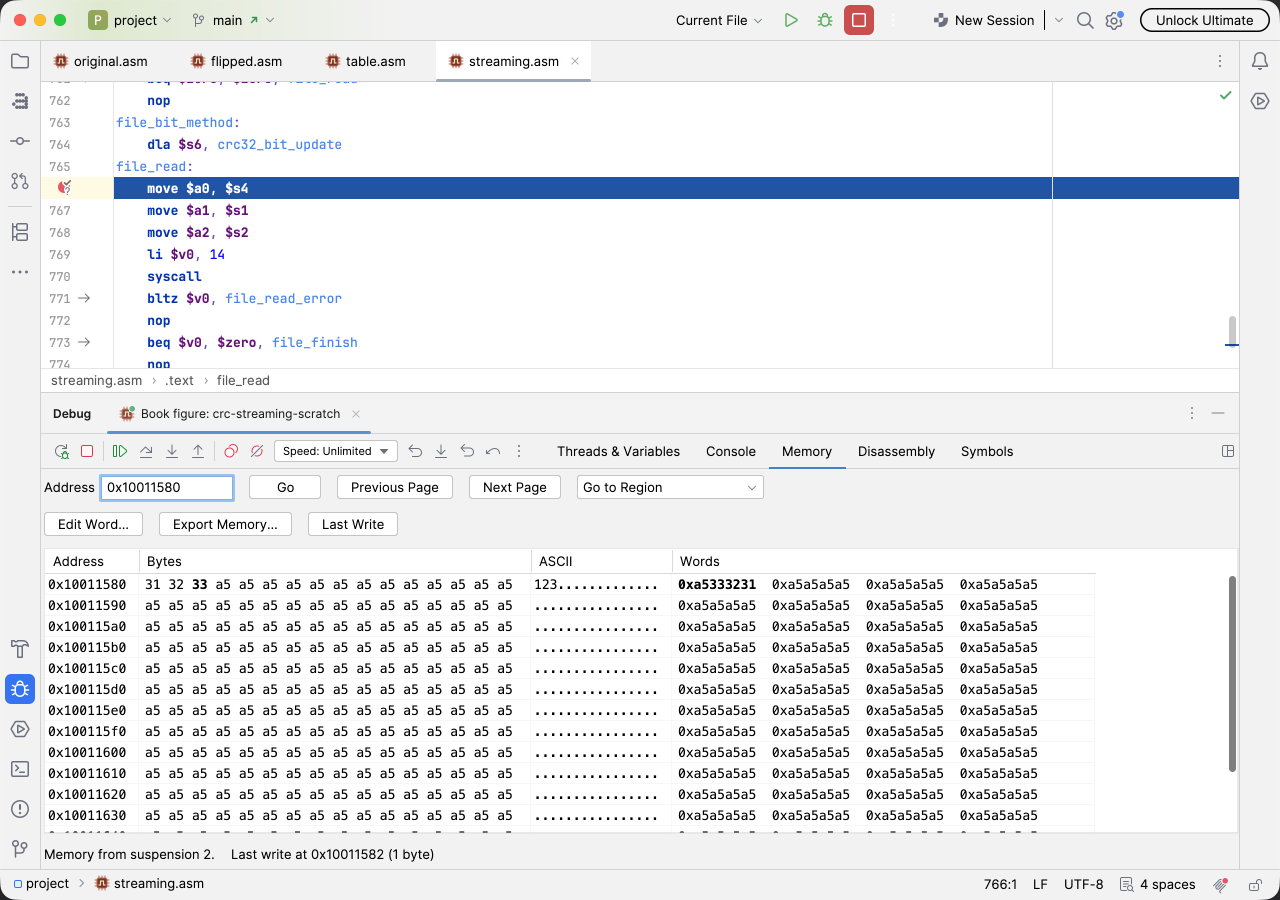
\includegraphics[artifact]{book/captures/024-crc32/f03/scratch.png}}
  \newsavebox{\MARScrcstreamingcontrolBox}
  \sbox{\MARScrcstreamingcontrolBox}{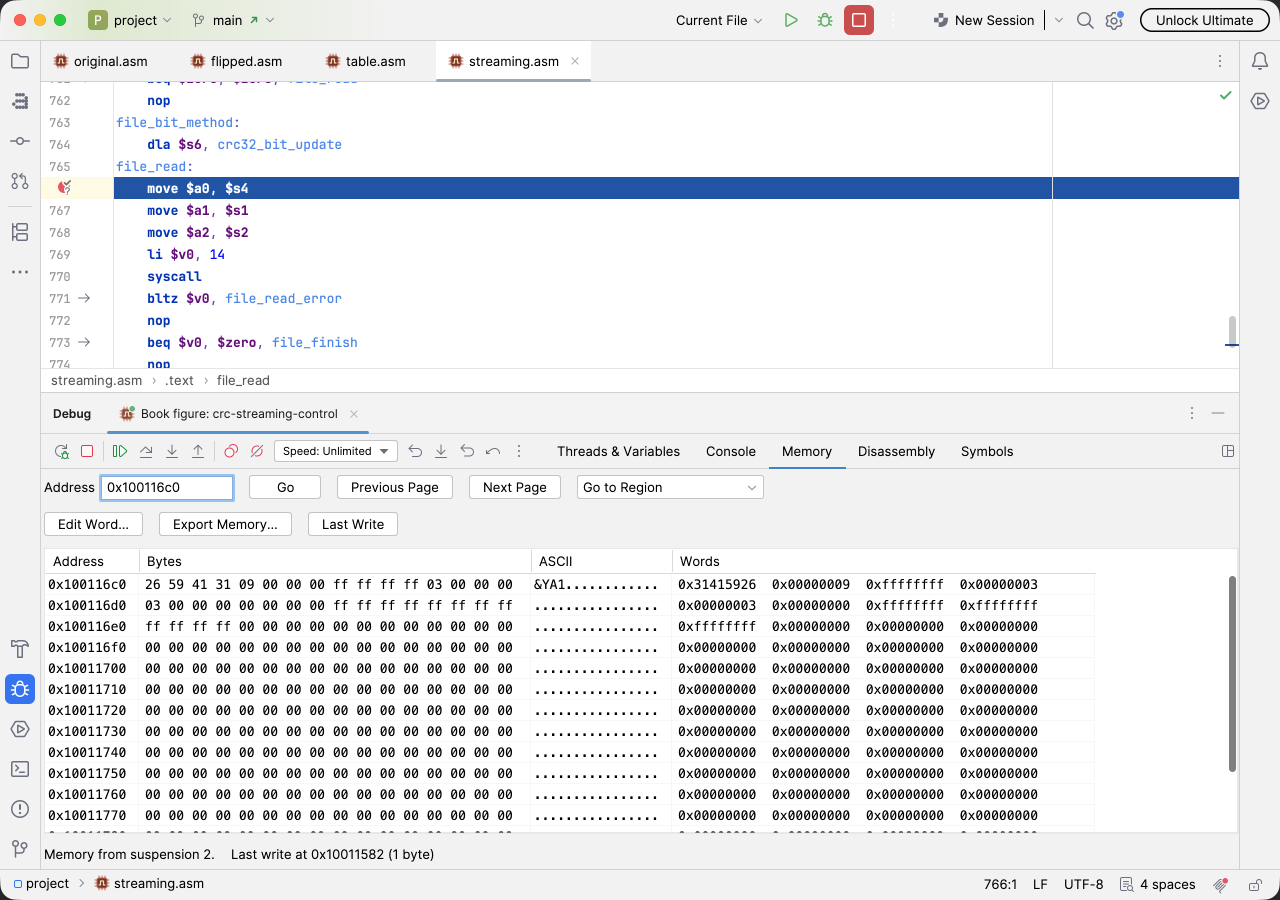
\includegraphics[artifact]{book/captures/024-crc32/f03/control.png}}
  \edef\MARScrcstreamingsourceLeft{\the\dimexpr0.036718750\wd\MARScrcstreamingregistersBox\relax}
  \edef\MARScrcstreamingsourceBottom{\the\dimexpr0.774444444\ht\MARScrcstreamingregistersBox\relax}
  \edef\MARScrcstreamingsourceRight{\the\dimexpr0.713281250\wd\MARScrcstreamingregistersBox\relax}
  \edef\MARScrcstreamingsourceTop{\the\dimexpr0.170000000\ht\MARScrcstreamingregistersBox\relax}
  \edef\MARScrcstreamingreturnsLeft{\the\dimexpr0.246093750\wd\MARScrcstreamingregistersBox\relax}
  \edef\MARScrcstreamingreturnsBottom{\the\dimexpr0.077777778\ht\MARScrcstreamingregistersBox\relax}
  \edef\MARScrcstreamingreturnsRight{\the\dimexpr0.553906250\wd\MARScrcstreamingregistersBox\relax}
  \edef\MARScrcstreamingreturnsTop{\the\dimexpr0.874444444\ht\MARScrcstreamingregistersBox\relax}
  \edef\MARScrcstreamingscratchLeft{\the\dimexpr0.034375000\wd\MARScrcstreamingscratchBox\relax}
  \edef\MARScrcstreamingscratchBottom{\the\dimexpr0.334444444\ht\MARScrcstreamingscratchBox\relax}
  \edef\MARScrcstreamingscratchRight{\the\dimexpr0.584375000\wd\MARScrcstreamingscratchBox\relax}
  \edef\MARScrcstreamingscratchTop{\the\dimexpr0.608888889\ht\MARScrcstreamingscratchBox\relax}
  \edef\MARScrcstreamingcontrolLeft{\the\dimexpr0.034375000\wd\MARScrcstreamingcontrolBox\relax}
  \edef\MARScrcstreamingcontrolBottom{\the\dimexpr0.311111111\ht\MARScrcstreamingcontrolBox\relax}
  \edef\MARScrcstreamingcontrolRight{\the\dimexpr0.584375000\wd\MARScrcstreamingcontrolBox\relax}
  \edef\MARScrcstreamingcontrolTop{\the\dimexpr0.608888889\ht\MARScrcstreamingcontrolBox\relax}
  \begin{tikzpicture}[alt={Four annotated details at the second file_read visit show open descriptor three and raw working state 77b79c2d. Scratch contains bytes 31 32 33 followed by unchanged a5 padding. The caller controls select capacity three and bit method zero; saved results remain minus one.}]
    \node[anchor=north west,inner sep=0,font=\small\bfseries] (source-title) at (6mm,0) {Next instruction at this boundary};
    \node[anchor=north west,inner sep=0] (source) at ([yshift=-1mm]source-title.south west) {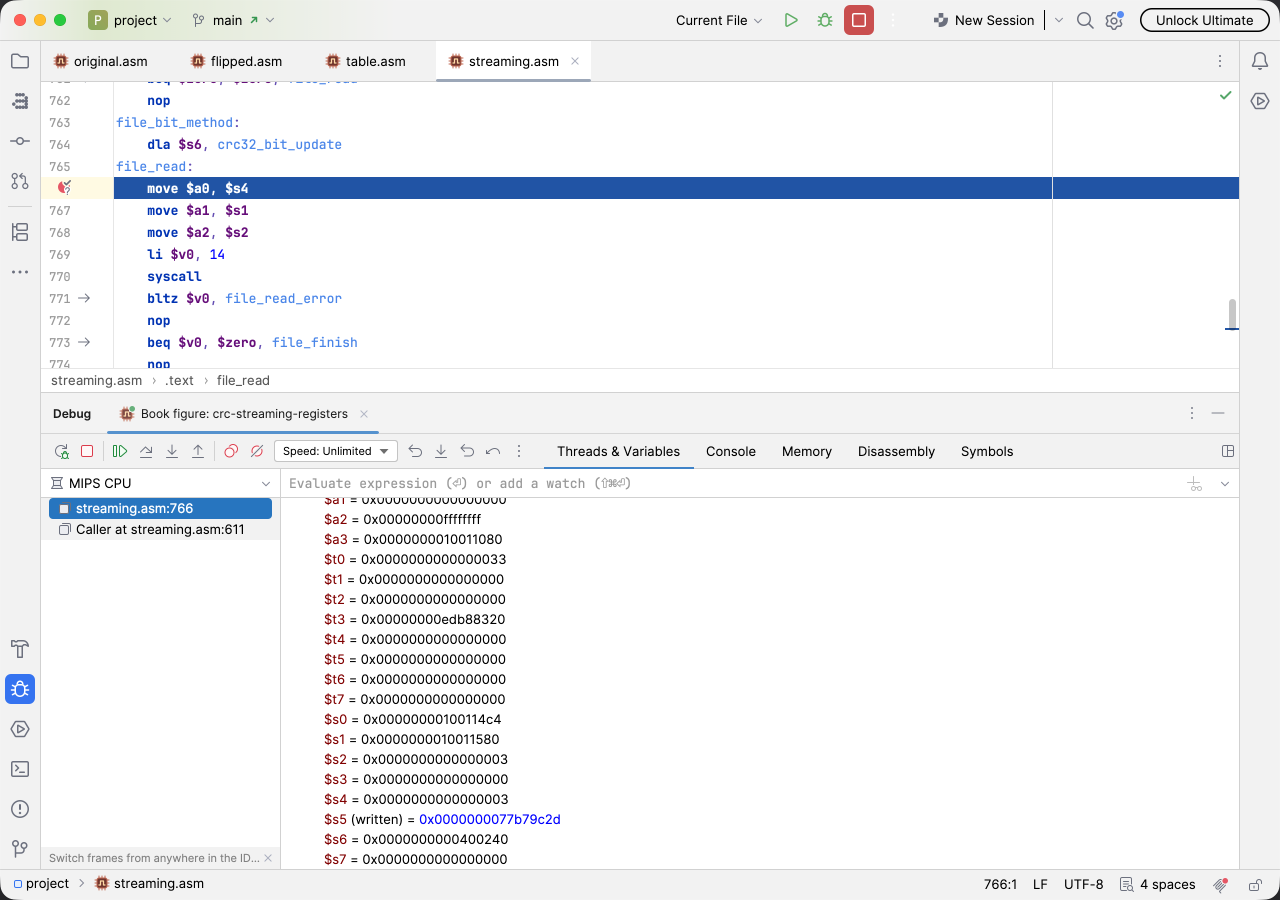
\includegraphics[width=0.54\linewidth,artifact,trim={\MARScrcstreamingsourceLeft{} \MARScrcstreamingsourceBottom{} \MARScrcstreamingsourceRight{} \MARScrcstreamingsourceTop{}},clip]{book/captures/024-crc32/f03/registers.png}};
    \begin{scope}[shift={(source.south west)},x={($(source.south east)-(source.south west)$)},y={($(source.north west)-(source.south west)$)}]
      \draw[black,line width=0.7pt] (0.215625000,0.080000000) rectangle (0.628125000,0.520000000);
      \node[draw=black,fill=white,circle,inner sep=1.5pt,font=\footnotesize] at ($(0.215625000,0.520000000)+(-3mm,0)$) {1};
    \end{scope}
    \node[anchor=north west,inner sep=0,font=\small\bfseries] (returns-title) at (0.58\linewidth,0 |- source-title.north) {Descriptor and working raw state};
    \node[anchor=north west,inner sep=0] (returns) at ([yshift=-1mm]returns-title.south west) {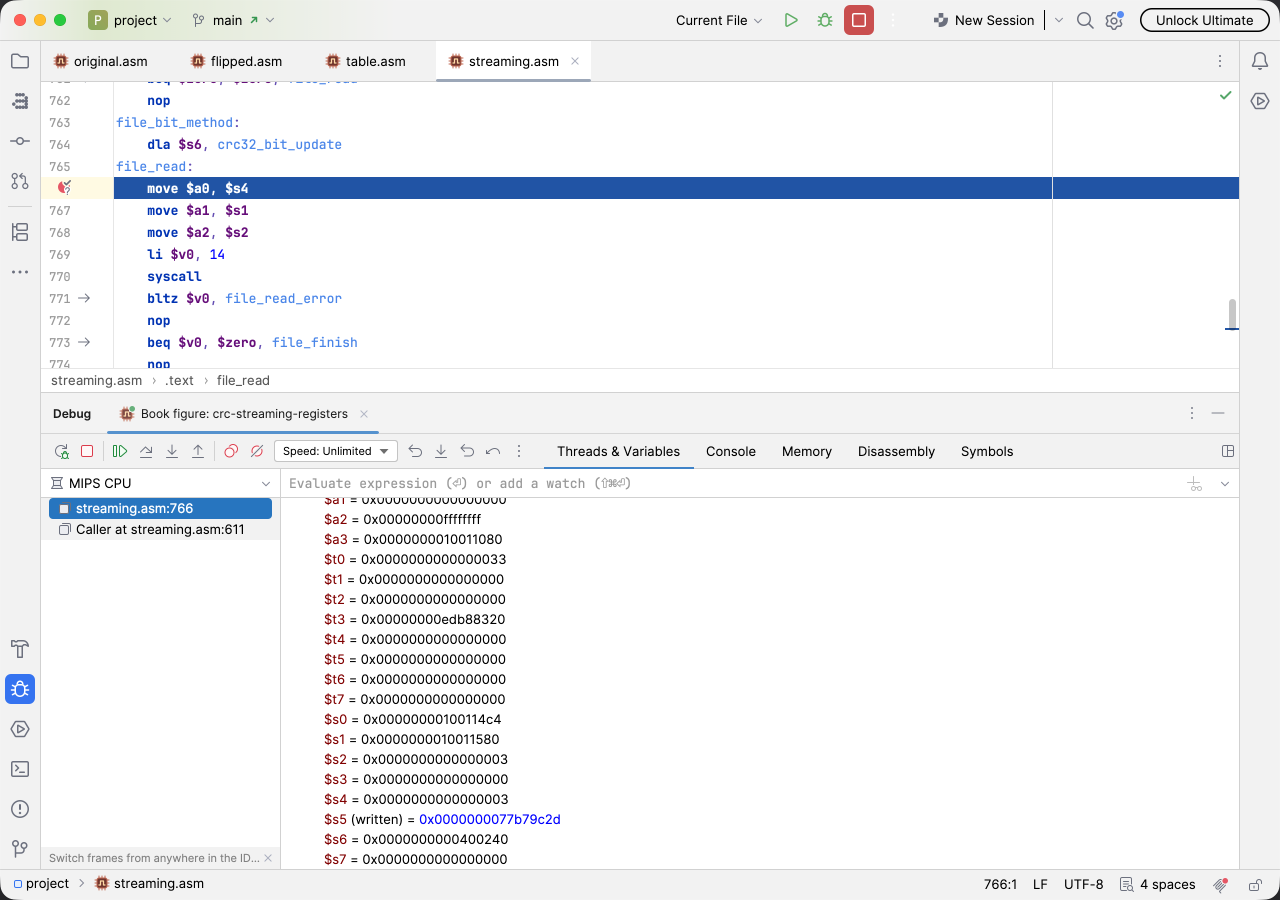
\includegraphics[width=0.42\linewidth,artifact,trim={\MARScrcstreamingreturnsLeft{} \MARScrcstreamingreturnsBottom{} \MARScrcstreamingreturnsRight{} \MARScrcstreamingreturnsTop{}},clip]{book/captures/024-crc32/f03/registers.png}};
    \begin{scope}[shift={(returns.south west)},x={($(returns.south east)-(returns.south west)$)},y={($(returns.north west)-(returns.south west)$)}]
      \draw[black,line width=0.7pt] (0.023437500,0.023255814) rectangle (0.964843750,0.953488372);
      \node[draw=black,fill=white,circle,inner sep=1.5pt,font=\footnotesize] at ($(0.023437500,0.953488372)+(-3mm,0)$) {2};
    \end{scope}
    \node[anchor=north west,inner sep=0,font=\small\bfseries] (scratch-title) at ([yshift=-1mm]source.south west) {Three-byte scratch prefix};
    \node[anchor=north west,inner sep=0] (scratch) at ([yshift=-1mm]scratch-title.south west) {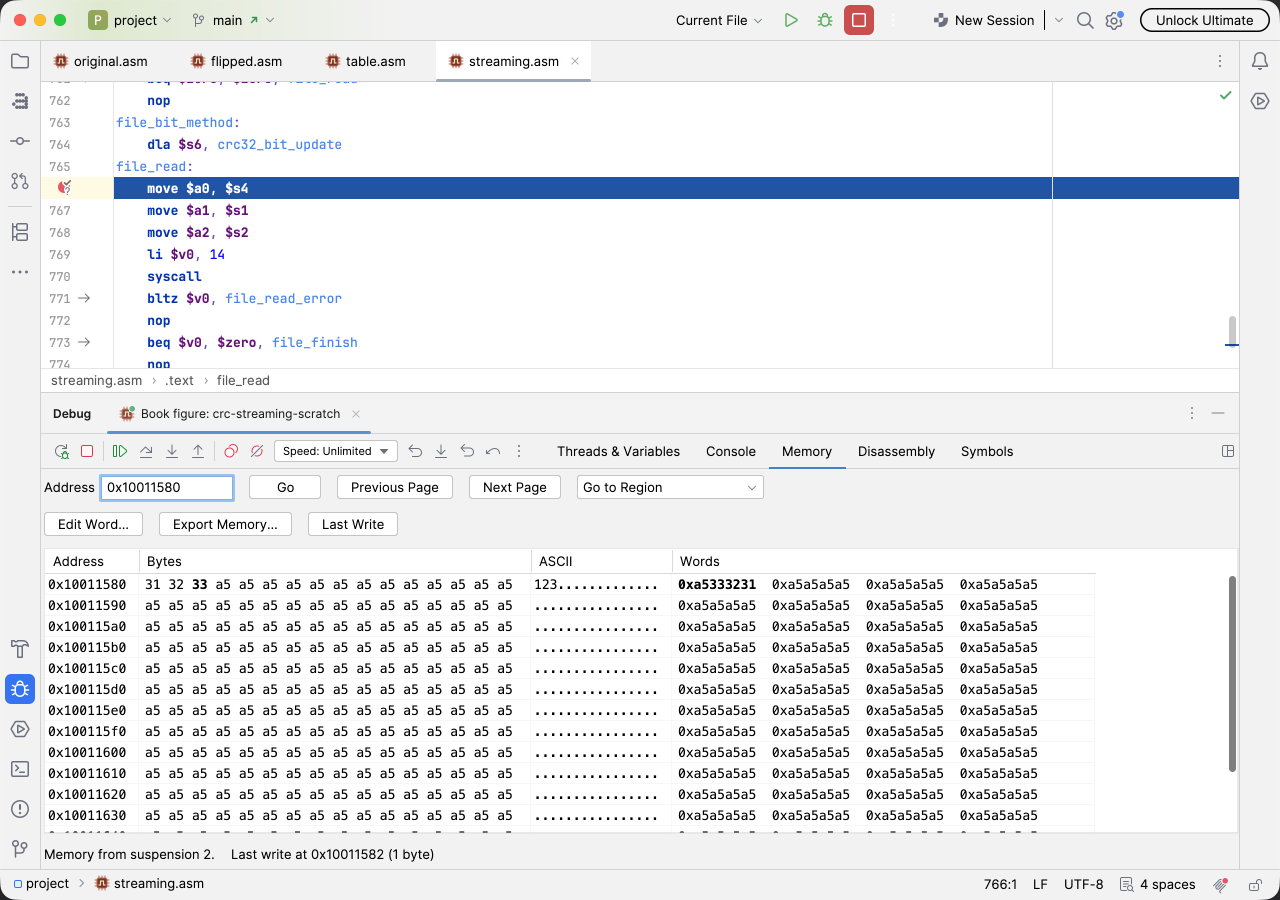
\includegraphics[width=0.84\linewidth,artifact,trim={\MARScrcstreamingscratchLeft{} \MARScrcstreamingscratchBottom{} \MARScrcstreamingscratchRight{} \MARScrcstreamingscratchTop{}},clip]{book/captures/024-crc32/f03/scratch.png}};
    \begin{scope}[shift={(scratch.south west)},x={($(scratch.south east)-(scratch.south west)$)},y={($(scratch.north west)-(scratch.south west)$)}]
      \draw[black,line width=0.7pt] (0.194672131,0.078431373) rectangle (0.997950820,0.490196078);
      \node[draw=black,fill=white,circle,inner sep=1.5pt,font=\footnotesize] at ($(0,0.490196078)+(-3mm,0)$) {3};
    \end{scope}
    \node[anchor=north west,inner sep=0,font=\small\bfseries] (control-title) at ([yshift=-1mm]scratch.south west) {Caller controls and saved results};
    \node[anchor=north west,inner sep=0] (control) at ([yshift=-1mm]control-title.south west) {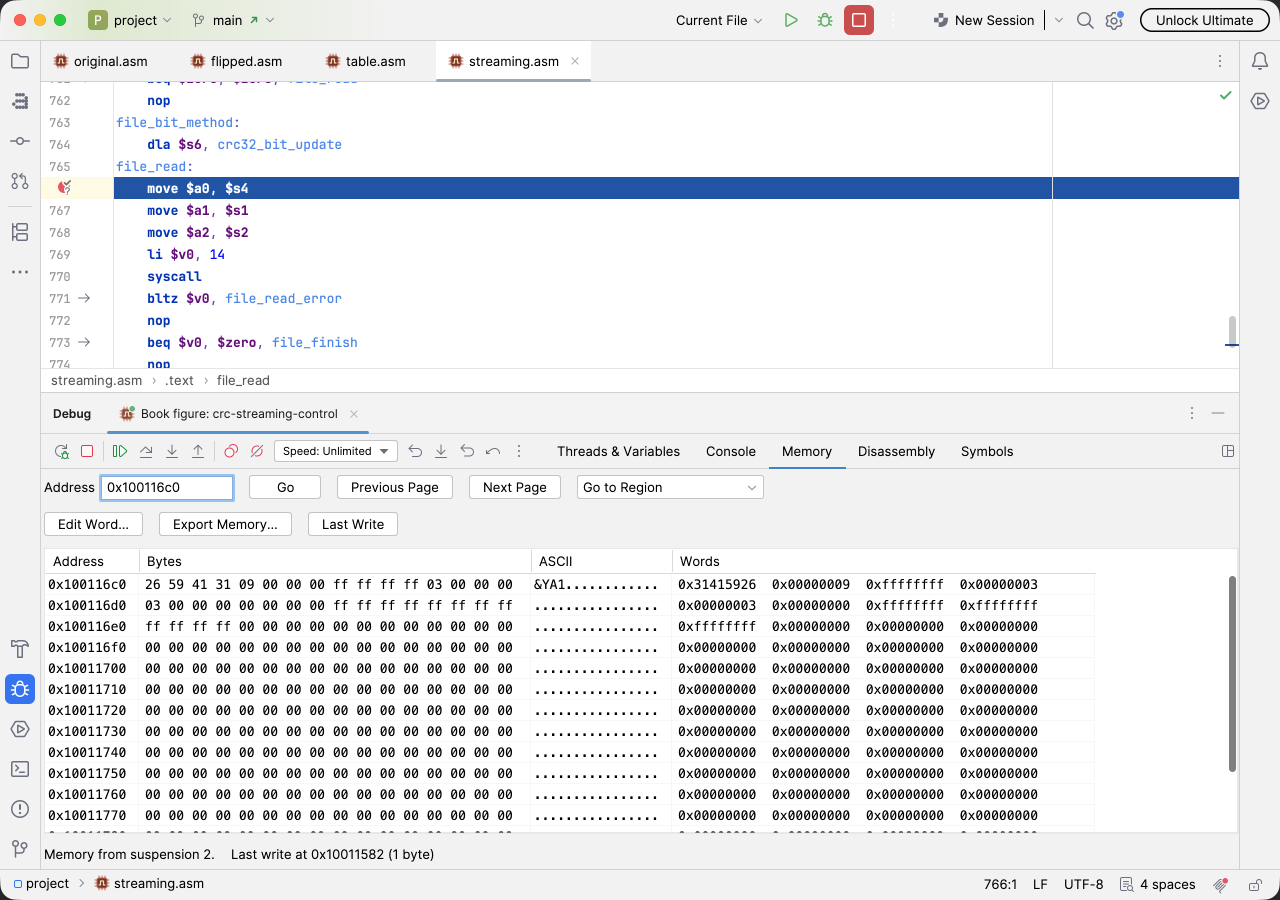
\includegraphics[width=0.84\linewidth,artifact,trim={\MARScrcstreamingcontrolLeft{} \MARScrcstreamingcontrolBottom{} \MARScrcstreamingcontrolRight{} \MARScrcstreamingcontrolTop{}},clip]{book/captures/024-crc32/f03/control.png}};
    \begin{scope}[shift={(control.south west)},x={($(control.south east)-(control.south west)$)},y={($(control.north west)-(control.south west)$)}]
      \draw[black,line width=0.7pt] (0.194672131,0.055555556) rectangle (0.997950820,0.638888889);
      \node[draw=black,fill=white,circle,inner sep=1.5pt,font=\footnotesize] at ($(0,0.638888889)+(-3mm,0)$) {4};
    \end{scope}
  \end{tikzpicture}
  \par\smallskip
  \begin{minipage}{\linewidth}
    \small
    \begin{enumerate}
      \setlength{\itemsep}{2pt}
            \setlength{\parsep}{0pt}
      \item The conditional stop is the second \texttt{file\_read} visit, before its next read syscall. After preparing the host-file recipe, set \texttt{buffer\_capacity} to three to reproduce this IDE view. Ordinary host reads then match the intended three-byte chunks without a forced short-read fixture.
      \item \texttt{s4 = 3} is this launch\textquotesingle s open descriptor, and \texttt{s5 = 0x77b79c2d} is raw state after \texttt{123}. Descriptor three is an observed value, not an interface requirement. Do not complement the state between chunks.
      \item Scratch begins \texttt{31 32 33}; its remaining bytes retain \texttt{a5}. Only the returned three bytes are consumed. Later reads replace the active prefix of this buffer rather than append to it.
      \item The controls show capacity three and bit method zero; saved result slots remain $-1$. Continuing processes \texttt{456} and \texttt{789}, then a zero-byte EOF read. Only then does the function complement the state, close its descriptor and return \texttt{cbf43926}, status zero.
    \end{enumerate}
  \end{minipage}
  \caption{Raw state remains uncomplemented between real three-byte file reads.}
  \label{capture:024-crc32-f03}
  \label{crc-f03}
\end{figure}
\par
